\section{Major scale}
\begin{definition}[Tetrachord]
    A 4-note scale segment with the following steps: $W-W-H$.
\end{definition}

\begin{definition}[Major scale]
    A 8-note scale made up of 2 tetrachords, joined by a whole step.
\end{definition}

$$\underbrace{W-W-H}_{T1}-W-\underbrace{W-W-H}_{T2}$$

\begin{figure}[h]
    \begin{center}
        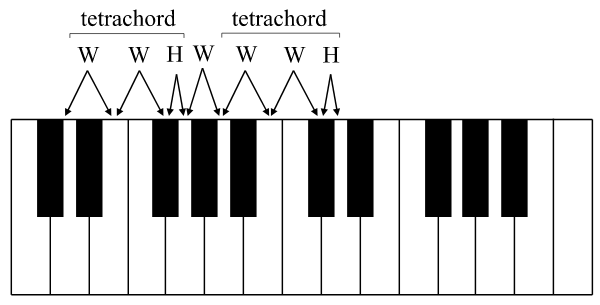
\includegraphics[width=0.6\textwidth]{img/tetrachord}
        \caption{Tetrachords in a (D) major scale}
    \end{center}
\end{figure}

A major scale uses all the 7 notes in order. No one is skipped and there are no duplicates.

\subsection{Key signatures}
There are 15 major key signatures:
\begin{itemize}
    \item 1 with no accidentals: C Major.
    \item 7 with $1$ to $7$ flats.
    \item 7 with $1$ to $7$ sharps.
\end{itemize}

\begin{figure}[h]
    \begin{center}
        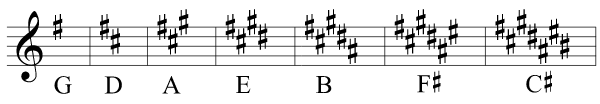
\includegraphics[width=0.8\textwidth]{img/majorsharp}
        \caption{Major key signatures (sharps)}
        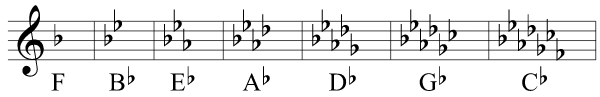
\includegraphics[width=0.8\textwidth]{img/majorflat}
        \caption{Major key signatures (flats)}
    \end{center}
\end{figure}
A key signature can be quickly identified with the following mnemonic:
\begin{itemize}
    \item With \emph{sharps}: +1 half step from the last ``sharped note''.
    \item With \emph{flats}: the second to last flat is the key (along with the flat).
\end{itemize}

\section{Minor scales}
\section{Circle of fifths}